\begin{figure}
\centering
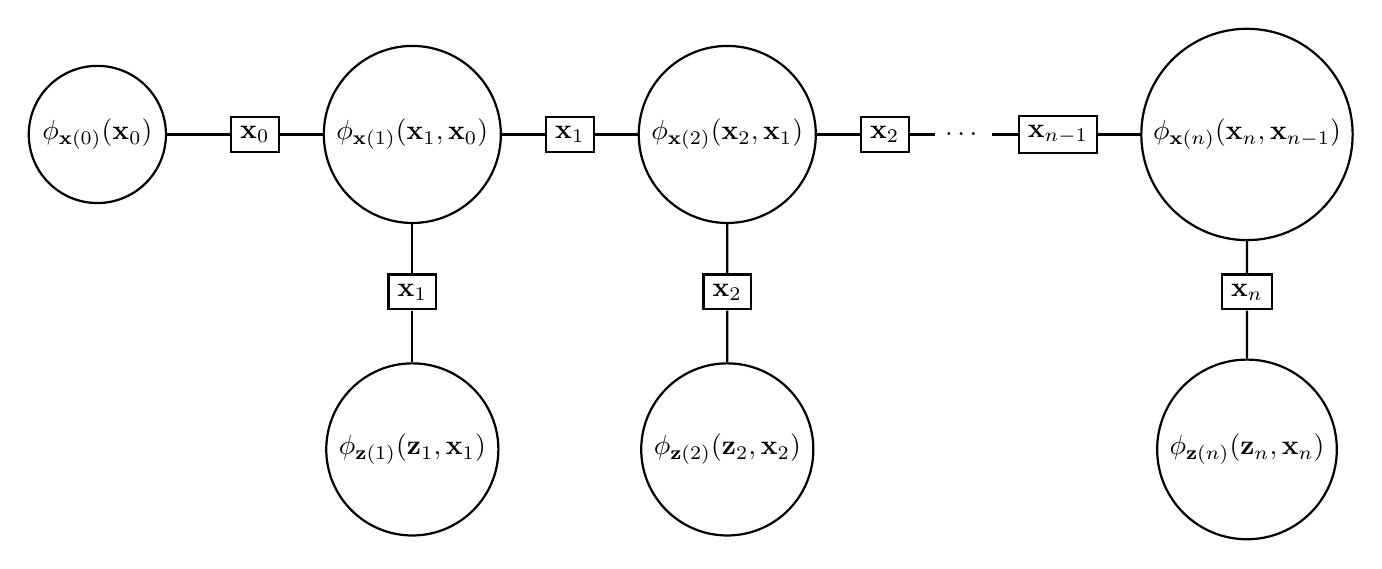
\begin{tikzpicture}[scale=0.80]
\begin{scope}[every node/.style={circle,thick,draw}]
	\node (x0) at (-5, 0) {$\phi_{\mathbf{x}{(0)}} (\mathbf{x}_{0})$};

    \node (x1) at (0, 0) {$\phi_{\mathbf{x}(1)} (\mathbf{x}_{1}, \mathbf{x}_{0})$};
    \node (z1) at (0, -5) {$\phi_{\mathbf{z}(1)} (\mathbf{z}_{1}, \mathbf{x}_{1})$};

    \node (xt) at (5, 0) {$\phi_{\mathbf{x}(2)} (\mathbf{x}_{2}, \mathbf{x}_{1})$};
    \node (zt) at (5, -5) {$\phi_{\mathbf{z}(2)} (\mathbf{z}_{2}, \mathbf{x}_{2})$};
    
    \node (xn) at (13.25, 0) {$\phi_{\mathbf{x}(n)} (\mathbf{x}_{n}, \mathbf{x}_{n-1})$};
    \node (zn) at (13.25, -5) {$\phi_{\mathbf{z}(n)} (\mathbf{z}_{n}, \mathbf{x}_{n})$};

\end{scope}

\begin{scope}[every node/.style={thick,draw}]
	\node (sx0) at (-2.5, 0) {$\mathbf{x}_{0}$};

    \node (sz1) at (0, -2.5) {$\mathbf{x}_{1}$};
    \node (sx1) at (2.5, 0) {$\mathbf{x}_{1}$};
    
    \node (szt) at (5, -2.5) {$\mathbf{x}_{2}$};
    \node (sxt) at (7.5, 0) {$\mathbf{x}_{2}$};
    
    \node (sxn) at (10.25,0) {$\mathbf{x}_{n-1}$};
    \node (szn) at (13.25, -2.5) {$\mathbf{x}_{n}$};
\end{scope}

\begin{scope}[style={thick,draw}]
    \node (xdot1) at (8.75,0) {\dots};
\end{scope}


\begin{scope}[style={thick,draw}]
	\path [-] (x0) edge node {} (sx0);
	\path [-] (sx0) edge node {} (x1);

	\path [-] (x1) edge node {} (sz1);
	\path [-] (sz1) edge node {} (z1);
	\path [-] (x1) edge node {} (sx1);
	\path [-] (sx1) edge node {} (xt);
	
	\path [-] (xt) edge node {} (szt);
	\path [-] (szt) edge node {} (zt);
	\path [-] (xt) edge node {} (sxt);
	\path [-] (sxt) edge node {} (xdot1);

	\path [-] (xdot1) edge node {} (sxn);	
	\path [-] (sxn) edge node {} (xn);
	\path [-] (xn) edge node {} (szn);	
	\path [-] (szn) edge node {} (zn);
	
\end{scope}

\end{tikzpicture}

\caption[Equivalent Junction Tree for a Kalman Filter.]{The Junction Tree  resulting  from the Bayes Net in Figure~\ref{figure:bayes_net}.}
\label{figure:junction_tree}
\end{figure}